\documentclass{beamer}
\usepackage{ctex, hyperref}
\usepackage[T1]{fontenc}

% 让数学公式更好看
\usefonttheme[onlymath]{serif}

\usepackage{indentfirst}
% \indent\setlength{\parindent}{1em}
\setlength{\parindent}{2em}


\newcommand\blfootnote[1]{%
  \begingroup
  \renewcommand\thefootnote{}\footnote{#1}%
  \addtocounter{footnote}{-1}%
  \endgroup
}

% other packages
\usepackage{latexsym,amsmath,xcolor,multicol,booktabs,calligra}
\usepackage{graphicx,pstricks,listings,stackengine}
\usepackage{epstopdf}
\usepackage{float}
\usepackage{multirow}

\usepackage{UESTC}


\title{Train BNNs with Reinforcement Learning}
\subtitle{毕业设计开题报告}
\author{唐国鑫}
\institute{四川师范大学数学科学学院}
\date{\today}


% defs
\def\cmd#1{\texttt{\color{red}\footnotesize $\backslash$#1}}
\def\env#1{\texttt{\color{blue}\footnotesize #1}}
\definecolor{deepblue}{rgb}{0,0,0.5}
\definecolor{deepred}{rgb}{0.6,0,0}
\definecolor{deepgreen}{rgb}{0,0.5,0}
\definecolor{halfgray}{gray}{0.55}

\lstset{
    basicstyle=\ttfamily\small,
    keywordstyle=\bfseries\color{deepblue},
    emphstyle=\ttfamily\color{deepred},    % Custom highlighting style
    stringstyle=\color{deepgreen},
    numbers=left,
    numberstyle=\small\color{halfgray},
    rulesepcolor=\color{red!20!green!20!blue!20},
    frame=shadowbox,
}


\begin{document}

\kaishu
\begin{frame}
    \titlepage
    \begin{figure}[htpb]
        \begin{center}
            
\includegraphics[width=0.2\linewidth]{pic/logo.pdf}
        \end{center}
    \end{figure}
\end{frame}

\begin{frame}
    \tableofcontents[sectionstyle=show,subsectionstyle=show/shaded/hide,subsubsectionstyle=show/shaded/hide]
\end{frame}


\section{课题背景}

\begin{frame}{Such A Huge Model}
    \footnotesize
    人工神经网络(ANN)是机器学习的主要研究对象之一. 早在$1958$年, Rosenblatt提出了感知机模型. 这是最早的ANN模型. 然而由于模型难以训练, 因此ANN并没有过多引起学者们的关注. 直到 $1986$年Hinton提出了反向传播算法(BP), 并且随着计算机算力的发展, ANN再次在机器学习领域掀起了研究热潮. 并衍生出了\textcolor{red}{深度学习}和\textcolor{red}{强化学习}领域. 而真正让人们记住深度学习和强化学习的威力的时间是$2016$年AlphaGo击败围棋世界冠军李世石, 并且在$2017$年再次击败围棋世界冠军柯洁. ANN强大的能力与它庞大而复杂的结构息息相关, 算法和算力的同时发展才使得训练出一个强大的ANN模型成为了可能.
\end{frame}

\begin{frame}{发展史}
    \footnotesize
    \begin{figure}
        \centering
        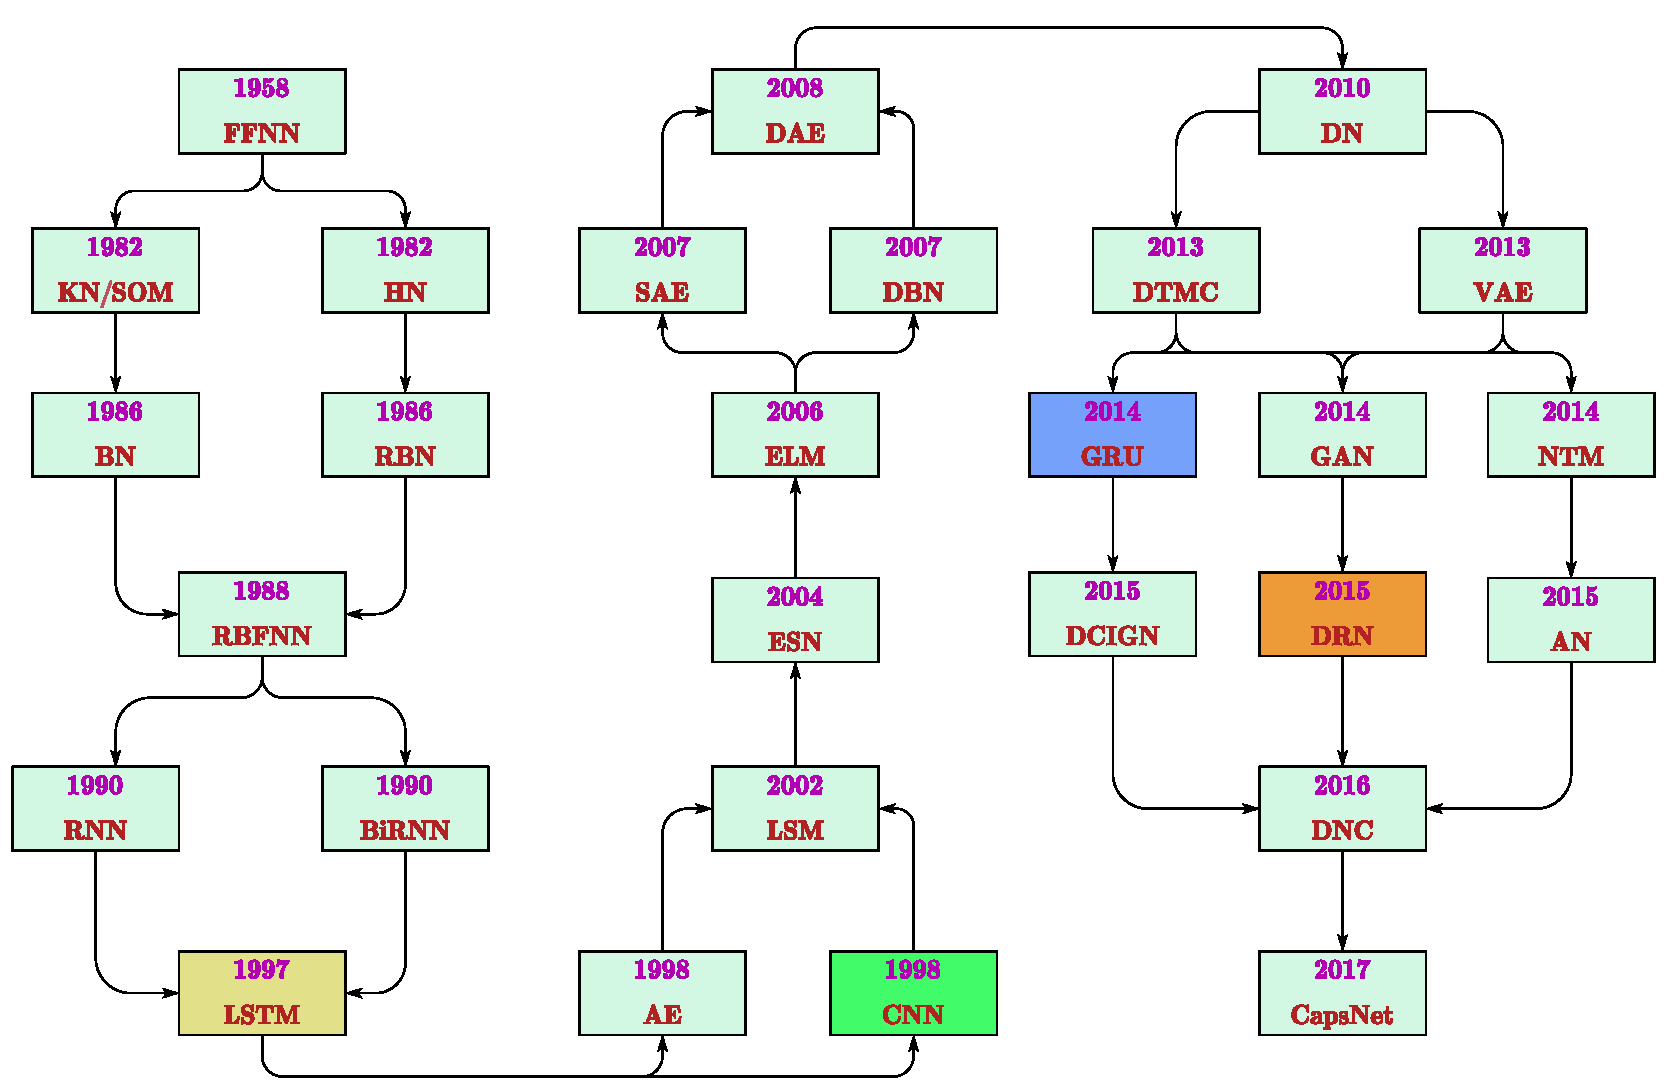
\includegraphics[scale=0.3]{pic/allnn.pdf}
    \end{figure}
\end{frame}

\begin{frame}{应用领域}
    \footnotesize
    \begin{columns}
        \column{0.5\textwidth}
        \begin{textbox}{\footnotesize 经典领域}
            \begin{enumerate}
                \item 时间序列分析
                \item 异常检测
                \item 图像及语音识别
                \item 数据挖掘及推荐系统
                \item 文本分类
                \item 微分方程求解, 分子及蛋白质结构预测
            \end{enumerate}
        \end{textbox}

        \column{0.5\textwidth}
        \begin{textbox}{\footnotesize 更多探索}
            \begin{enumerate}
                \item 上下文知识推理
                \item 数学逻辑和定理证明
                \item 根据注释进行代码补全
                \item 图形风格迁移
                \item 视频画质修复和补帧
                \item 自动玩游戏, 写诗
            \end{enumerate}
        \end{textbox}
        
    \end{columns}
    
\end{frame}

\begin{frame}{Such A Huge Model}
    \footnotesize
    $1998$年Yann LeCun提出了LeNet-5\cite{lenet5nn}模型, 并在手写数字识别上获得成功. LeNet-5不是卷积神经网络(CNN)的起点, 但却是CNN兴起的标志. 图\ref{fig:lenet5}是LeNet-5的结构. 它一共有 $122~304$ 个参数.
    \begin{figure}
        \centering
        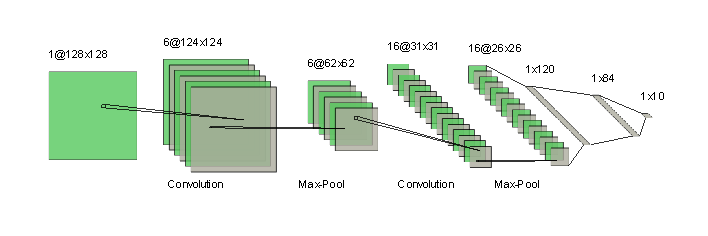
\includegraphics[scale=0.8]{./pic/lenet5.pdf}
        \caption{{LeNet-5}}
        \label{fig:lenet5}
    \end{figure}
\end{frame}

\begin{frame}{Such A Huge Model}
    \begin{table}[H]
        \centering
        \caption{经典的CNN构架}
        \vspace{-0.3cm}
        \label{tab:cnns}
        % \resizebox{\textwidth}{!}{%
        \begin{tabular}{ccccc}
        \hline
        Name       & Year & Author            & Depth & Parameter            \\ \hline
        LeNet-5    & $1998$ & LeCun             & $7$     & $122~304$              \\
        AlexNet    & $2012$ & Alex \& Jeffry     & $9$     & $60~965~128$          \\
        VGGNet     & $2014$ & Oxford university & $16$    & $138~357~544$ \\
        GoogleNet  & $2014$ & Google            & $22$    & $6~994~392$            \\
        ResNet     & $2015$ & Microsoft(何凯明等人)  & $168$   & $25~636~712$  \\
        Xception   & $2017$ & Chollet           & $126$   & $22~910~480$           \\
        MobileNets & $2017$ & Google            & $88$    & $4~253~864$            \\
        PaLM       & $2022$ & Google            & $118$     & $540.35$ billions                \\ \hline
        \end{tabular}%
        % }
        \end{table}
\end{frame}

\begin{frame}{Such A Huge Model}
    \footnotesize
    然而, 训练一个如此庞大的模型的代价在实际应用中很多时候是难以接受的. 以PaLM模型为例, Google共用了$6144$块TPU(Tensor Processing Unit)来进行训练. 强大的系统和算力带来了惊艳的结果, 也产生了巨大的资源消耗. 此外, 杨迪一\cite{wang2021gnn}等人在论文中的实验证明, 在GNN中, 可能有$99\%$的参数都是冗余的. 我们有理由怀疑是否模型中所有的参数都是必要的. 

    另一方面, 庞大的模型很难嵌入到我们的小型设备(如智能手机, 智能手表等). 对模型进行瘦身是有必要的.

\end{frame}

\begin{frame}{Such A Huge Model}
    \footnotesize
    图\ref{fig:fit26}是$f(x) = x^2 + \mathcal{N}(0,1)$生成的数据.
    \begin{figure}[H]
        \centering
        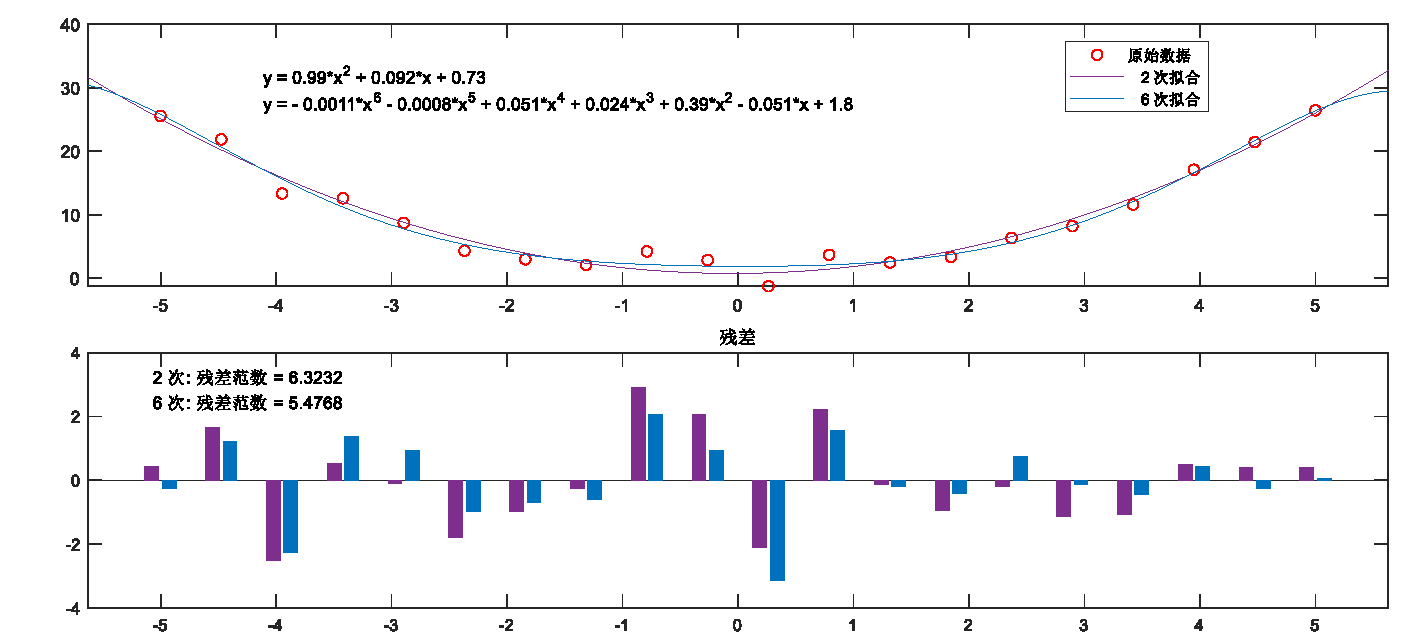
\includegraphics[scale=0.4]{pic/morepar.pdf}
        \caption{二次多项式拟合与六次多项式拟合}
        \label{fig:fit26}
    \end{figure}
\end{frame}


\section{研究现状}

\begin{frame}{知识蒸馏}
    知识蒸馏\cite{hinton2015distilling}最早于2015年由Hinton提出, 蒸馏的目的是为了缩减模型. 此外也有蒸馏特征的数据蒸馏\cite{wang2018dataset}. 通过蒸馏的手段, 使得模型变小或数据集更加易于学习, 以此到达降低训练成本的目的.
    \begin{itemize}
        \item 模型剪枝
        \item 量化
        \item 参数共享
    \end{itemize}
\end{frame}

\begin{frame}{量化}
    \footnotesize
    我们的主要研究集中在模型的量化上, 比如用$8$位浮点数代替$32$位浮点数, 或将浮点数向上或向下取整为一个整数等. 模型量化的主要方法有:
    \begin{itemize}
        \item 二值化网络: Binary Network \cite{courbariaux2015binaryconnect}
        \item 三值化网络: Ternary Network \cite{li2016ternary}
        \item 深度压缩: Deep Compression \cite{han2015deep}
    \end{itemize}
    此外, 对模型的压缩或缩减不局限于使用一种方法, 多数时候会结合量化与剪枝等操作在一个模型上.
    
\end{frame}

\begin{frame}{Binary Neural Networks(BNNs)}
    \footnotesize
    $2015$年, Bengio\cite{courbariaux2015binaryconnect}等人第一次将神经网络中的参数二值化, 并在MINST, CIFAR-10和SVHN数据集上达到了SOTA级别的性能. Bengio对网络量化的可行性的解析如下:
    \begin{itemize}
        \item 对参数的量化其实是对参数引入了一定程度的噪声, 并在训练过程中通过累计逐渐被平均掉.
        \item 类似于DropOut和DropConnect, 参数引入噪声意味着给网路施加了某种正则成分, 从而提高网络的泛化性能.
    \end{itemize}
    通过对参数的量化, 使得原来浮点数的乘法运算变成了加法运算甚至直接使用位运算, 这不仅大大降低了模型所需要的物理内存, 也极大提高了计算效率.
    \blfootnote{\noindent \tiny{值得一提的是, Hinton, LeCun和Bengio三人一起获得了2018年国际计算机协会(ACM)图灵奖}}
\end{frame}

\begin{frame}{阻碍}
    \footnotesize
    然而白璧微瑕. 二值化量化带来了低内存, 高效率的优势的同时, 也引发了一系列新的问题. 由于权重的值域不再连续, 面临的第一个困难就是BNNs的梯度处处为$0$. 这使得Hinton的反向传播算法无法直接对BNNs生效. 

    $2012$年, Hinton提出直通估计器(Straight Through Estimator: STE)\cite{bengio2013estimating}. 网络的前向传播使用被量化的$w_b$来计算, 但是仍然保留全精度的原始$w$用于计算梯度. 下面的公式是文中参数二值化的方法.
    \begin{equation}
        w_b=\mathrm{sign}(w)=\begin{cases}
            +1&		w\geqslant 0\\
            -1&		\mathrm{otherwise}\\
        \end{cases}
    \end{equation}
\end{frame}


\begin{frame}{方案}
	\footnotesize
    为了解决参数二值化后梯度处处为$0$, 泛化性能降低等问题, 许多学者从以下方面对BNNs进行了研究\cite{qin2020binary}:
    \begin{itemize}
        \item 使用新的预定义函数对权重进行量化
        \item 通过最小量化误差来逼近全精度值
        \item 修改损失函数来限制权重
        \item 减小梯度误差来学习离散参数
    \end{itemize}
    \begin{figure}[H]
        \centering
        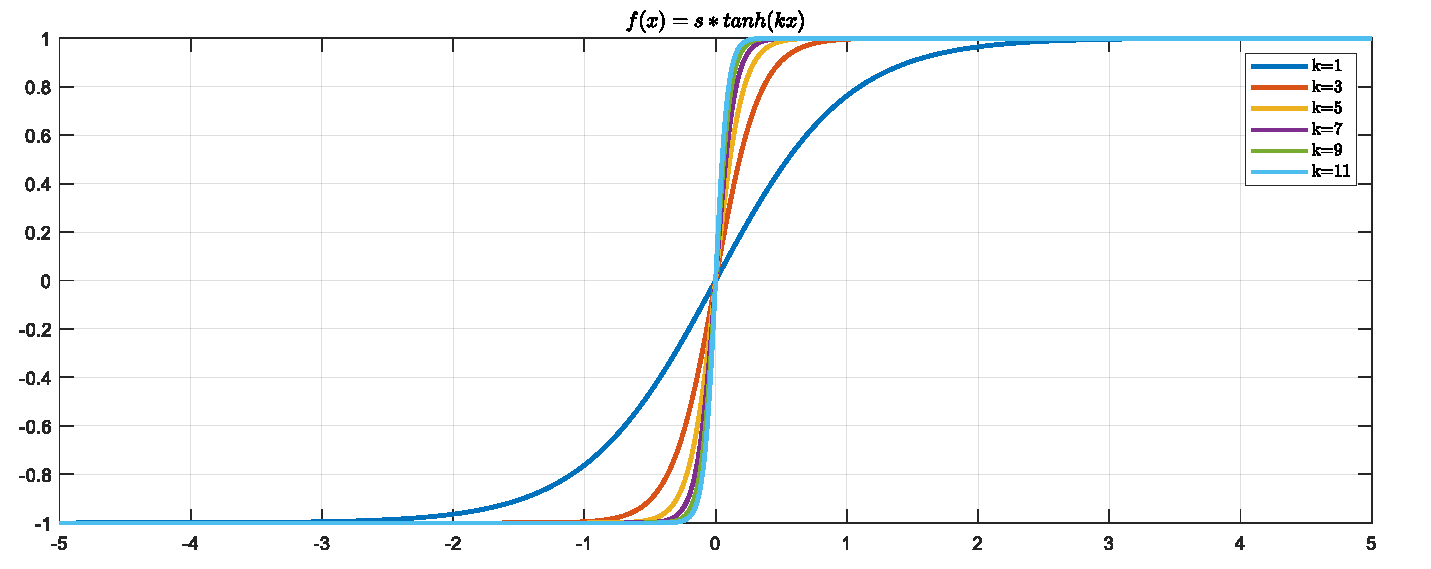
\includegraphics[scale=0.2]{pic/appro.pdf}
        \caption{量化逼近}
    \end{figure}
\end{frame}

\begin{frame}{方案}
	\footnotesize
    下面的方法分别是部分对损失函数的修改, 使用量化误差逼近全精度权重以及减少梯度误差的方法.
    \begin{figure}[H]
        \centering
        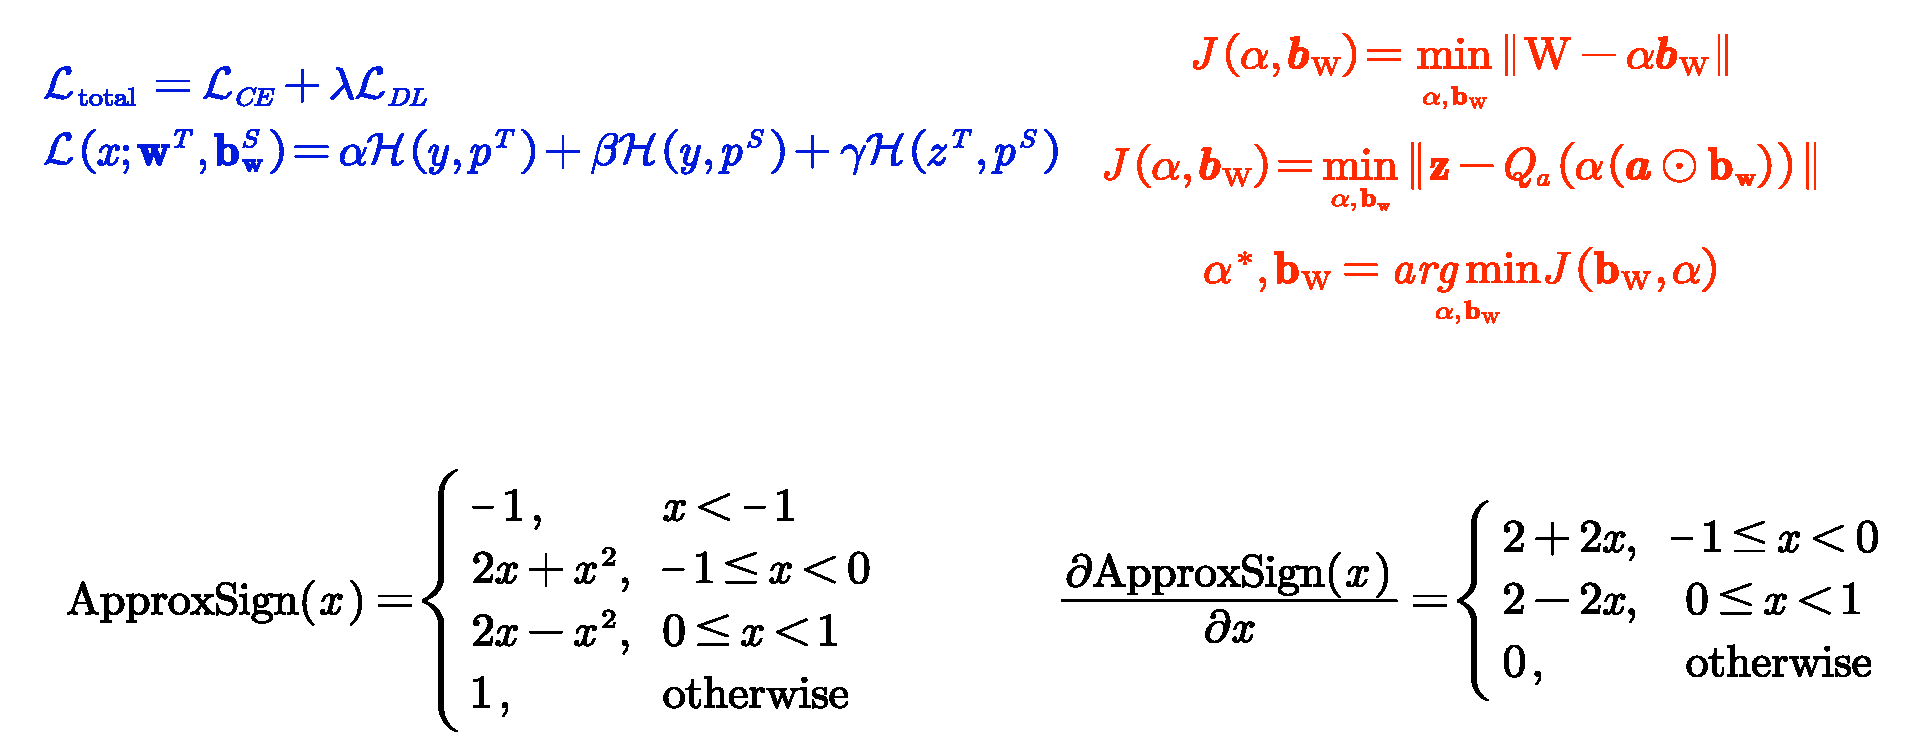
\includegraphics[scale=0.3]{pic/m3.pdf}
        \caption{已有的部分方案}
    \end{figure}
\end{frame}

\begin{frame}{方案}
\footnotesize
自$2015$年以来, 已查阅到的BNNs新的研究已多达$36$种. 下表给出了部分已有的对BNNs的研究, 它们都是基于以上思想对BNNs新的探索.
% Please add the following required packages to your document preamble:
% \usepackage{multirow}
% \usepackage{graphicx}
\begin{table}[H]
    \centering
    \footnotesize
    \caption{部分基于这些方法所提出的新模型}
    \vspace*{-0.3cm}
    \label{tab:impmode}
    % \resizebox{\textwidth}{!}{%
    \begin{tabular}{ccc}
    \hline
    Type                     & Method                     & Key Tech.          \\ \hline
    \multirow{3}{*}{朴素BNNs}  & BinaryConnect              & \multirow{3}{*}{STE} \\
                             & Bitwise Neural Networks    &                    \\
                             & Binarized Neural Networks  &                    \\ \hline
    \multirow{3}{*}{最小化量化误差} & Binary Weight Networks    & \multirow{3}{*}{$ \alpha ^*,\mathbf{b}_{\mathrm{W}}=\underset{\alpha ,\mathbf{b}_{\mathrm{W}}}{arg\min}J\left( \mathbf{b}_{\mathrm{W}},\alpha \right)  $} \\
                             & XNOR-Net                   &                    \\
                             & DoReFa-Net                 &                    \\ \hline
    \multirow{3}{*}{改进损失函数}  & BNN-DL                     & \multirow{3}{*}{$\mathcal{L} _{\mathrm{total}}=\mathcal{L} _{CE}+\lambda \mathcal{L} _{DL}$} \\
                             & CI-BCNN                    &                    \\
                             & Loss-Aware Binarization    &                    \\ \hline
    \multirow{3}{*}{减少梯度误差}  & BNN+                       & \multirow{3}{*}{$\varphi \left( x \right) =s\tanh \left( kx \right) $} \\
                             & BCGD   &                    \\
                             & IR-NET &                    \\ \hline
    \end{tabular}%
    % }
    \end{table}
\end{frame}


\begin{frame}{无法回避的问题}
    \footnotesize
    总的来说, 几乎所有对BNNs的探索都集中如何处理梯度处处为$0$的问题. 目的就是为了使得误差的反向传播能够重新工作起来. STE尽管可以一定程度上可以让我们重新使用SGD, Adam等算法进行训练. 然而, 二值化参数对梯度的大小是不敏感的. 这可能导致下面的情况产生:
    \begin{equation}
        \begin{matrix}
            \mathrm{sign}(+1-\nabla _w)=+1~(\nabla _w=-1,-10)\\
            \mathrm{sign}(-1-\nabla _w)=-1~(\nabla _w=-1,-10).\\
        \end{matrix}
    \end{equation} 
    换句话说, 达到一定大小值的梯度对参数的改变不再起决定性作用. 我们应该更加关心的是梯度的方向或梯度的动作, 而不是梯度的值.
\end{frame}

\section{研究内容}

\begin{frame}{优化方法}
    \footnotesize
    在梯度可求且不处处为$0$的情况下, SGD, Adam, L-BFGS等算法是训练BNNs的不错选择. 如果将BNNs模型写作下面的形式:
    \begin{equation}
        \begin{matrix}
            \mathcal{L} =\max -\mathcal{L} \left( \mathrm{W}_b \right)\\
            s.t.~w_{b\left( i,j \right)}=-1~\mathrm{or}~1.\\
        \end{matrix}
    \end{equation}
    我们可以将其看做一个非线性整数规划问题(当参数为$0$和$1$时, 也可以看做是$0,1$整数规划或指派问题). 然而, 常规的割平面法和分支定界法无法使用. 遗传算法(GA)是解决这一问题的一种可行方案. 但是庞大的参数会给GA的搜索进化带来困难, 甚至难以收敛到一个令人满意的局部最优值. 并且迭代时间可能也是难以让人接受的. 
\end{frame}

\begin{frame}{非梯度不可吗?}
    \footnotesize
    如果我们一定要用基于梯度的算法来训练BNNs, 我们就不得不向寻找梯度的代替方案屈服. 如果要用基于无梯度方法的算法(如GA), 我们就要付出更多的时间代价甚至牺牲模型的精度. 
    
    已有的对BNNs梯度为$0$的研究都是在想办法如何使得反向传播重新工作. 在我们的研究中, 我们不再将梯度当做梯度, 也不再需要梯度来调整我们的参数. 而是将参数的调整看作是一个动作的调整. 这是就是强化学习的基本观点之一. 强化学习是最接近人的学习行为方式的算法.
\end{frame}

\begin{frame}{动机}
    \footnotesize
    考虑一个如下的走迷宫问题: 机器人从左上角出发, 且只能上下左右移动, 需要从绿色的出口离开. 机器人每走一步, 就会得到$-1$分的奖励, 掉入红色的陷阱中则游戏结束, 需要重新从起点出发. 而到达出口则可以获得$100$分的奖励. 那么我们需要考虑的就是如何最大化自己的奖励.
    \begin{figure}
        \centering
        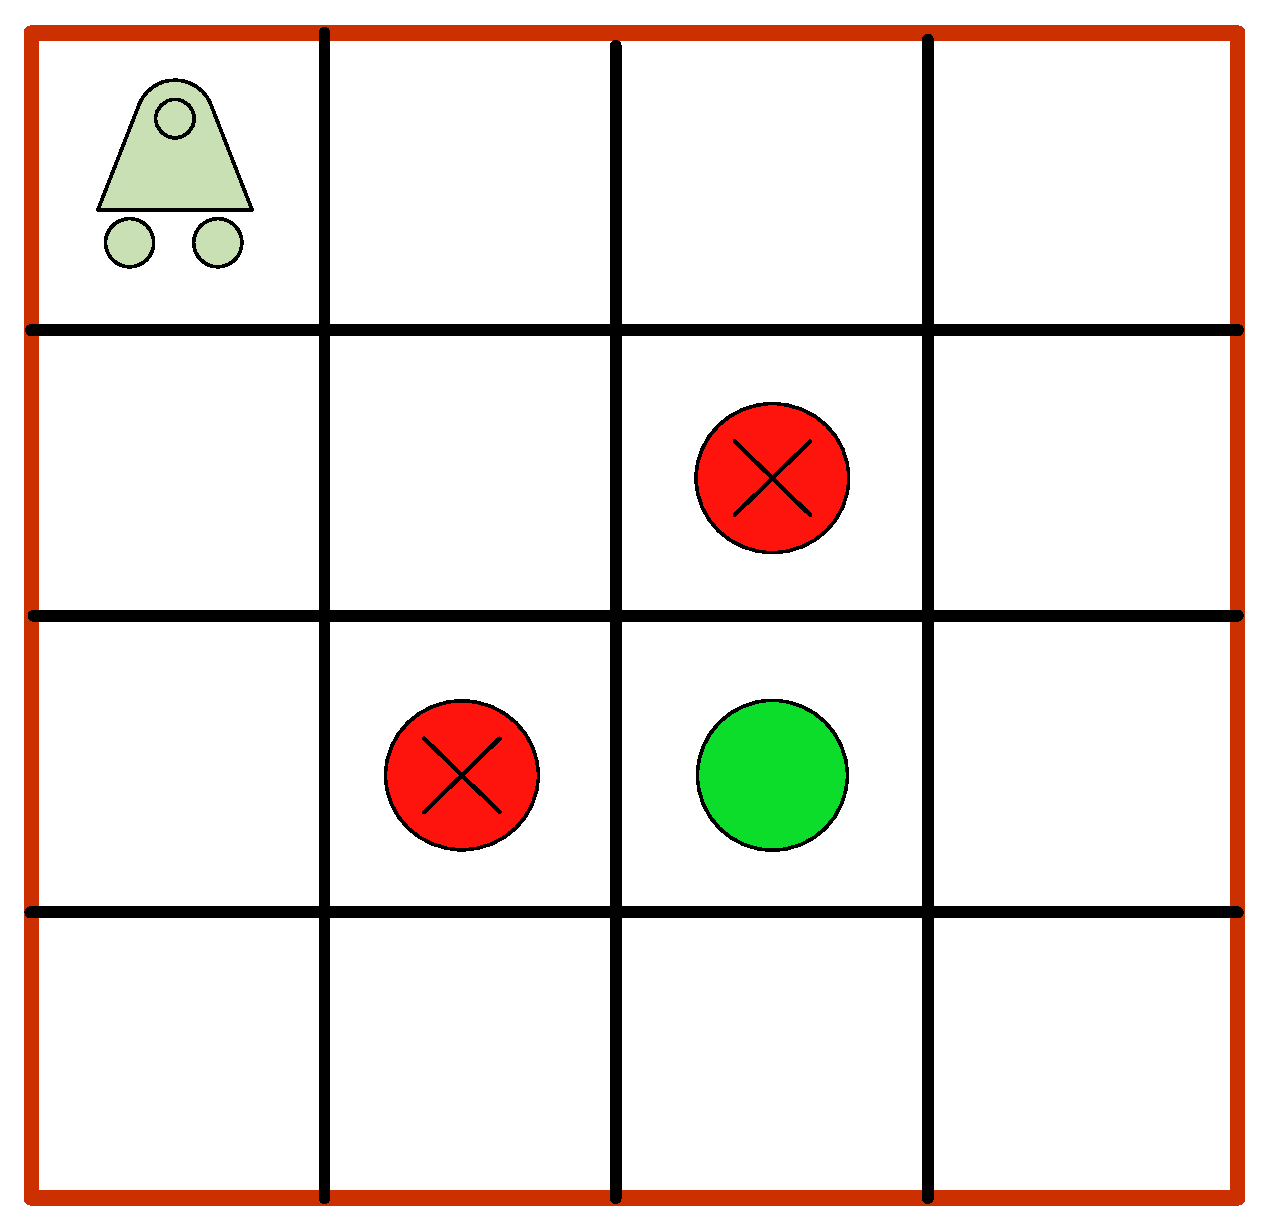
\includegraphics[scale=0.2]{pic/maze.pdf}
        \caption{Maze}
        \label{fig:maze}
    \end{figure}
\end{frame}

\begin{frame}{动机}
    \footnotesize
    比较传统的方法如DFS和BFS算法, 我们都可以直接找到到达出口的最优方案或策略. 然而在强化学习中, 我们会让机器人找到在每一个位置(或状态)价值最大的动作. 在图\ref{fig:maze2}中, 通过观察可以发现想要最快到达, 应该向右移动. 确定处于任意位置的最大价值的动作是强化学习的目标.
    \begin{figure}
        \centering
        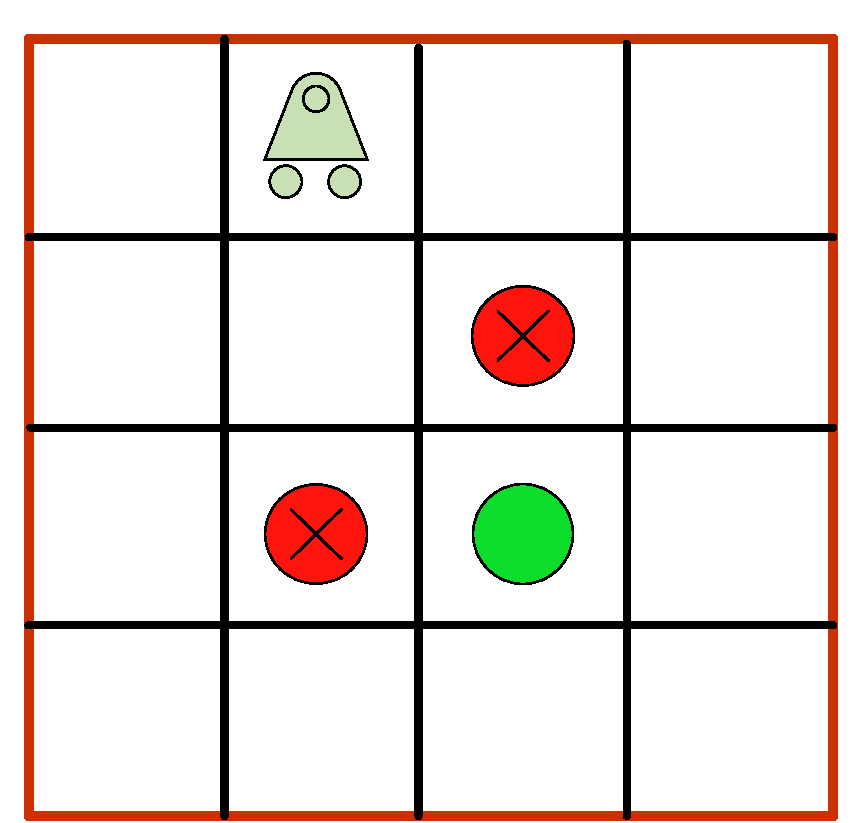
\includegraphics[scale=0.3]{pic/maze2.pdf}
        \caption{处于某一个状态的机器人}
        \label{fig:maze2}
    \end{figure}
\end{frame}

\begin{frame}{强化学习}
    \footnotesize
    下图是强化学习的基本示意图. 本文将BNNs的训练看作是一个强化学习过程. 从而不直接使用梯度的方法来更新BNNs的参数. 图中展示了强化学习的$5$个基本元素.
    \begin{figure}
        \centering
        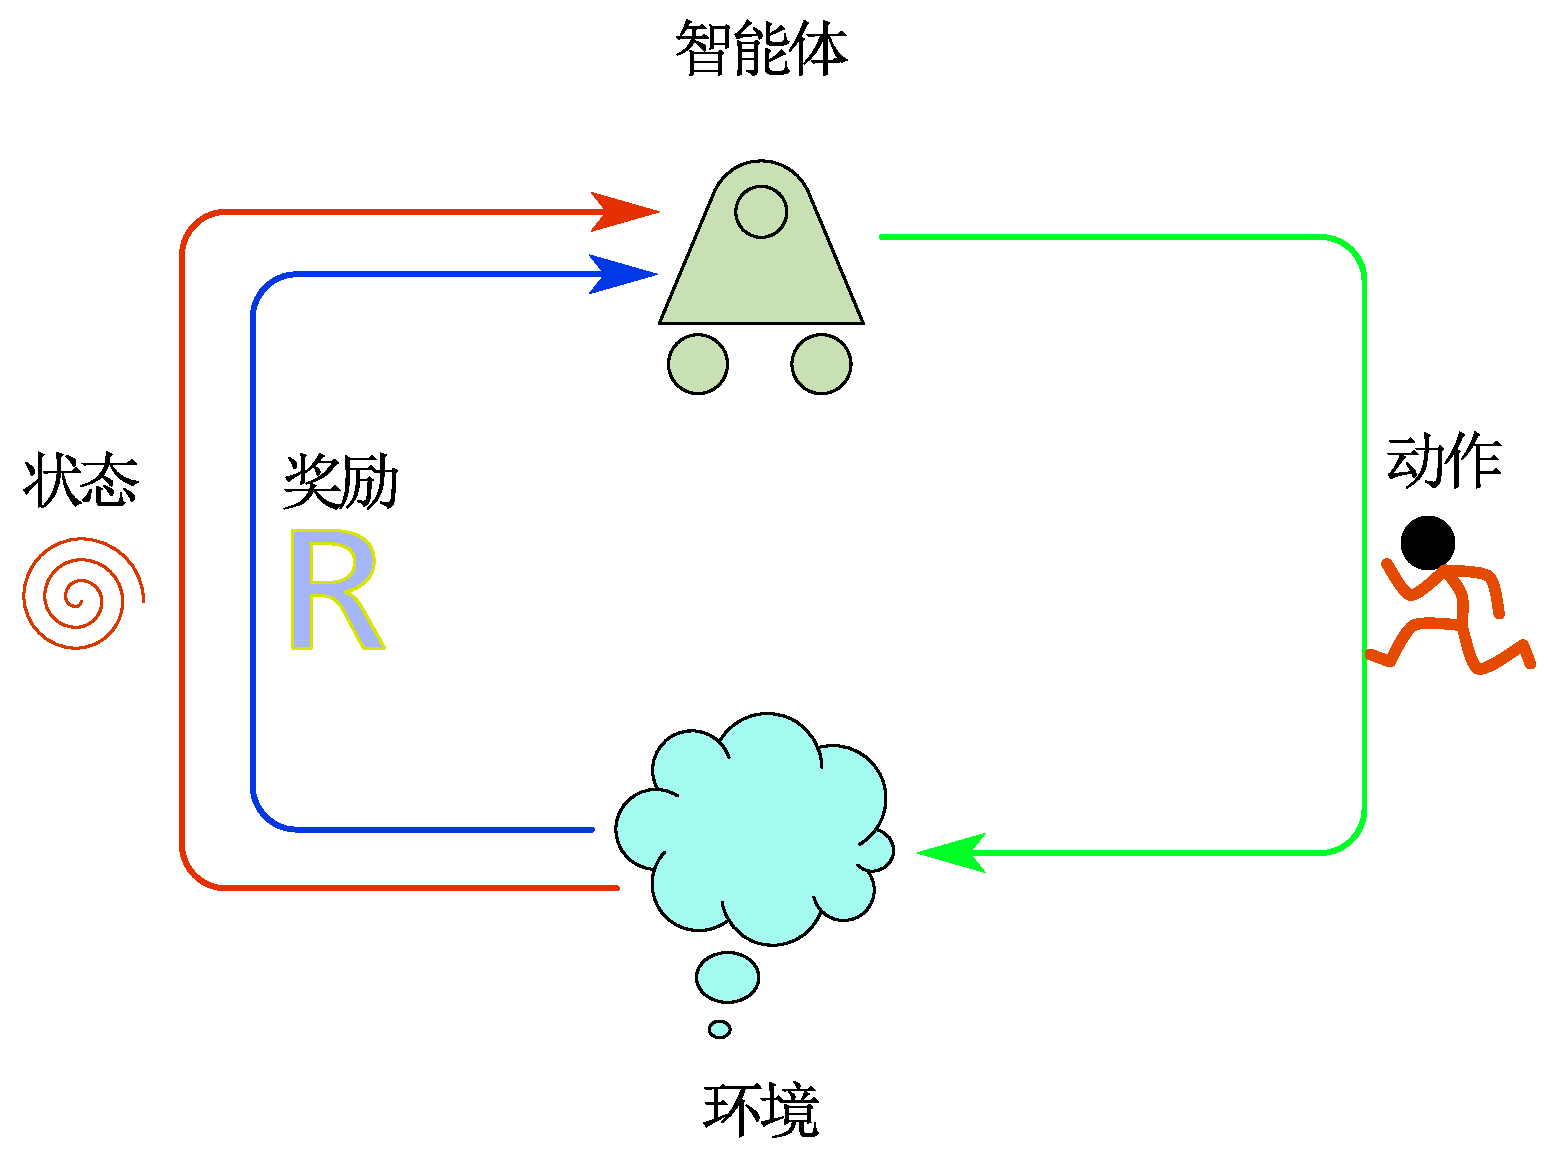
\includegraphics[scale=0.3]{pic/rl.pdf}
        \caption{强化学习基本过程}
        \label{fig:RL}
    \end{figure}
\end{frame}

\begin{frame}{强化学习}
    \footnotesize
    强化学习的目的是找到一个最优的动作策略, 价值函数用于评价动作的好坏. 而在训练BNNs的过程中, 则是通过学习动作找到一个最优的状态使得价值函数最大.
    \begin{figure}
        \centering
        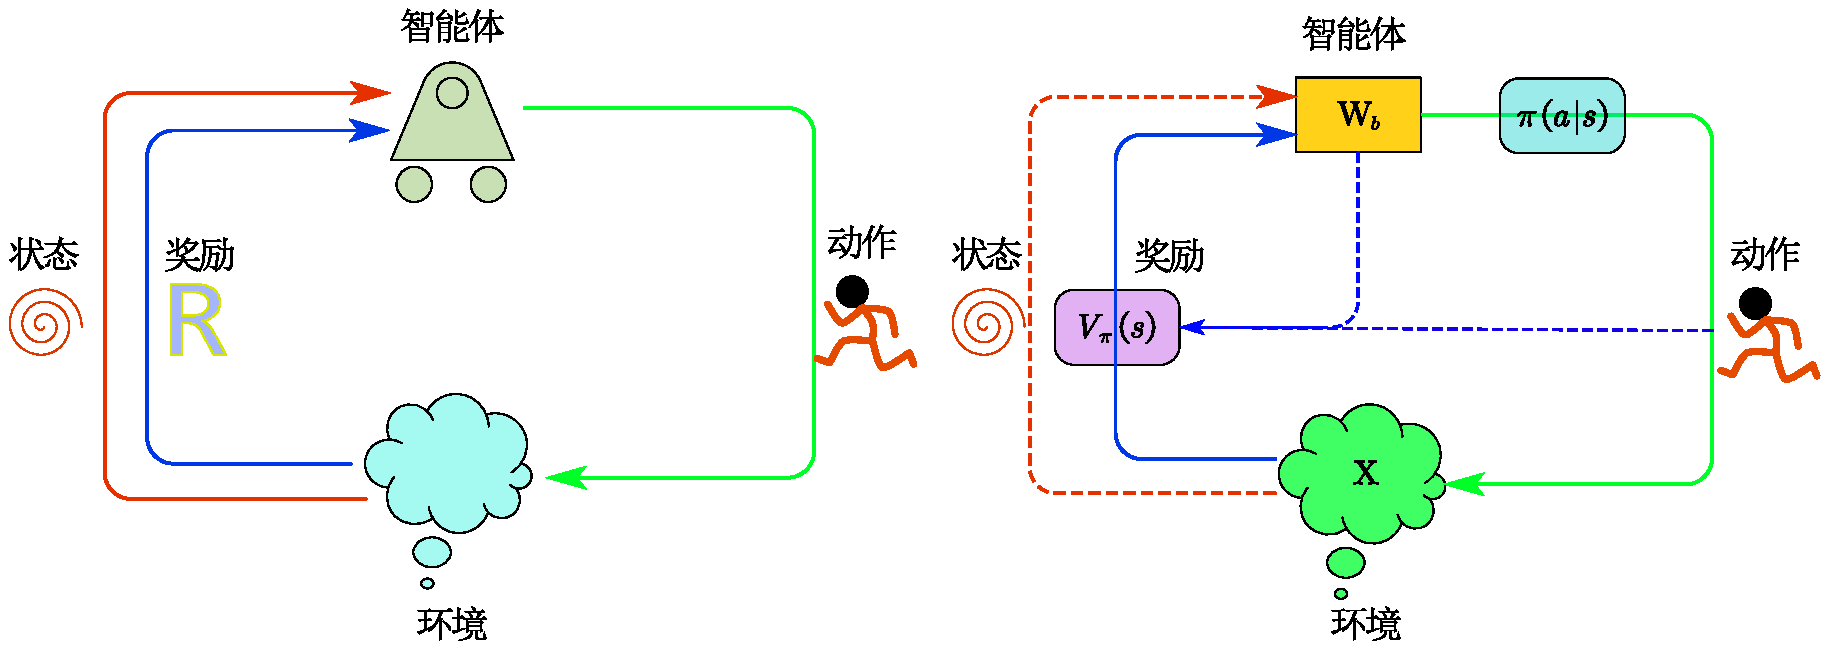
\includegraphics[scale=0.35]{pic/cmp1.pdf}
        \caption{强化学习下的BNNs}
    \end{figure}
\end{frame}


\begin{frame}{调整动作的一个列子}
    \footnotesize
    下图展示了如何调整动作来使得直线将两个类别分离出来.
    \begin{figure}
        \centering
        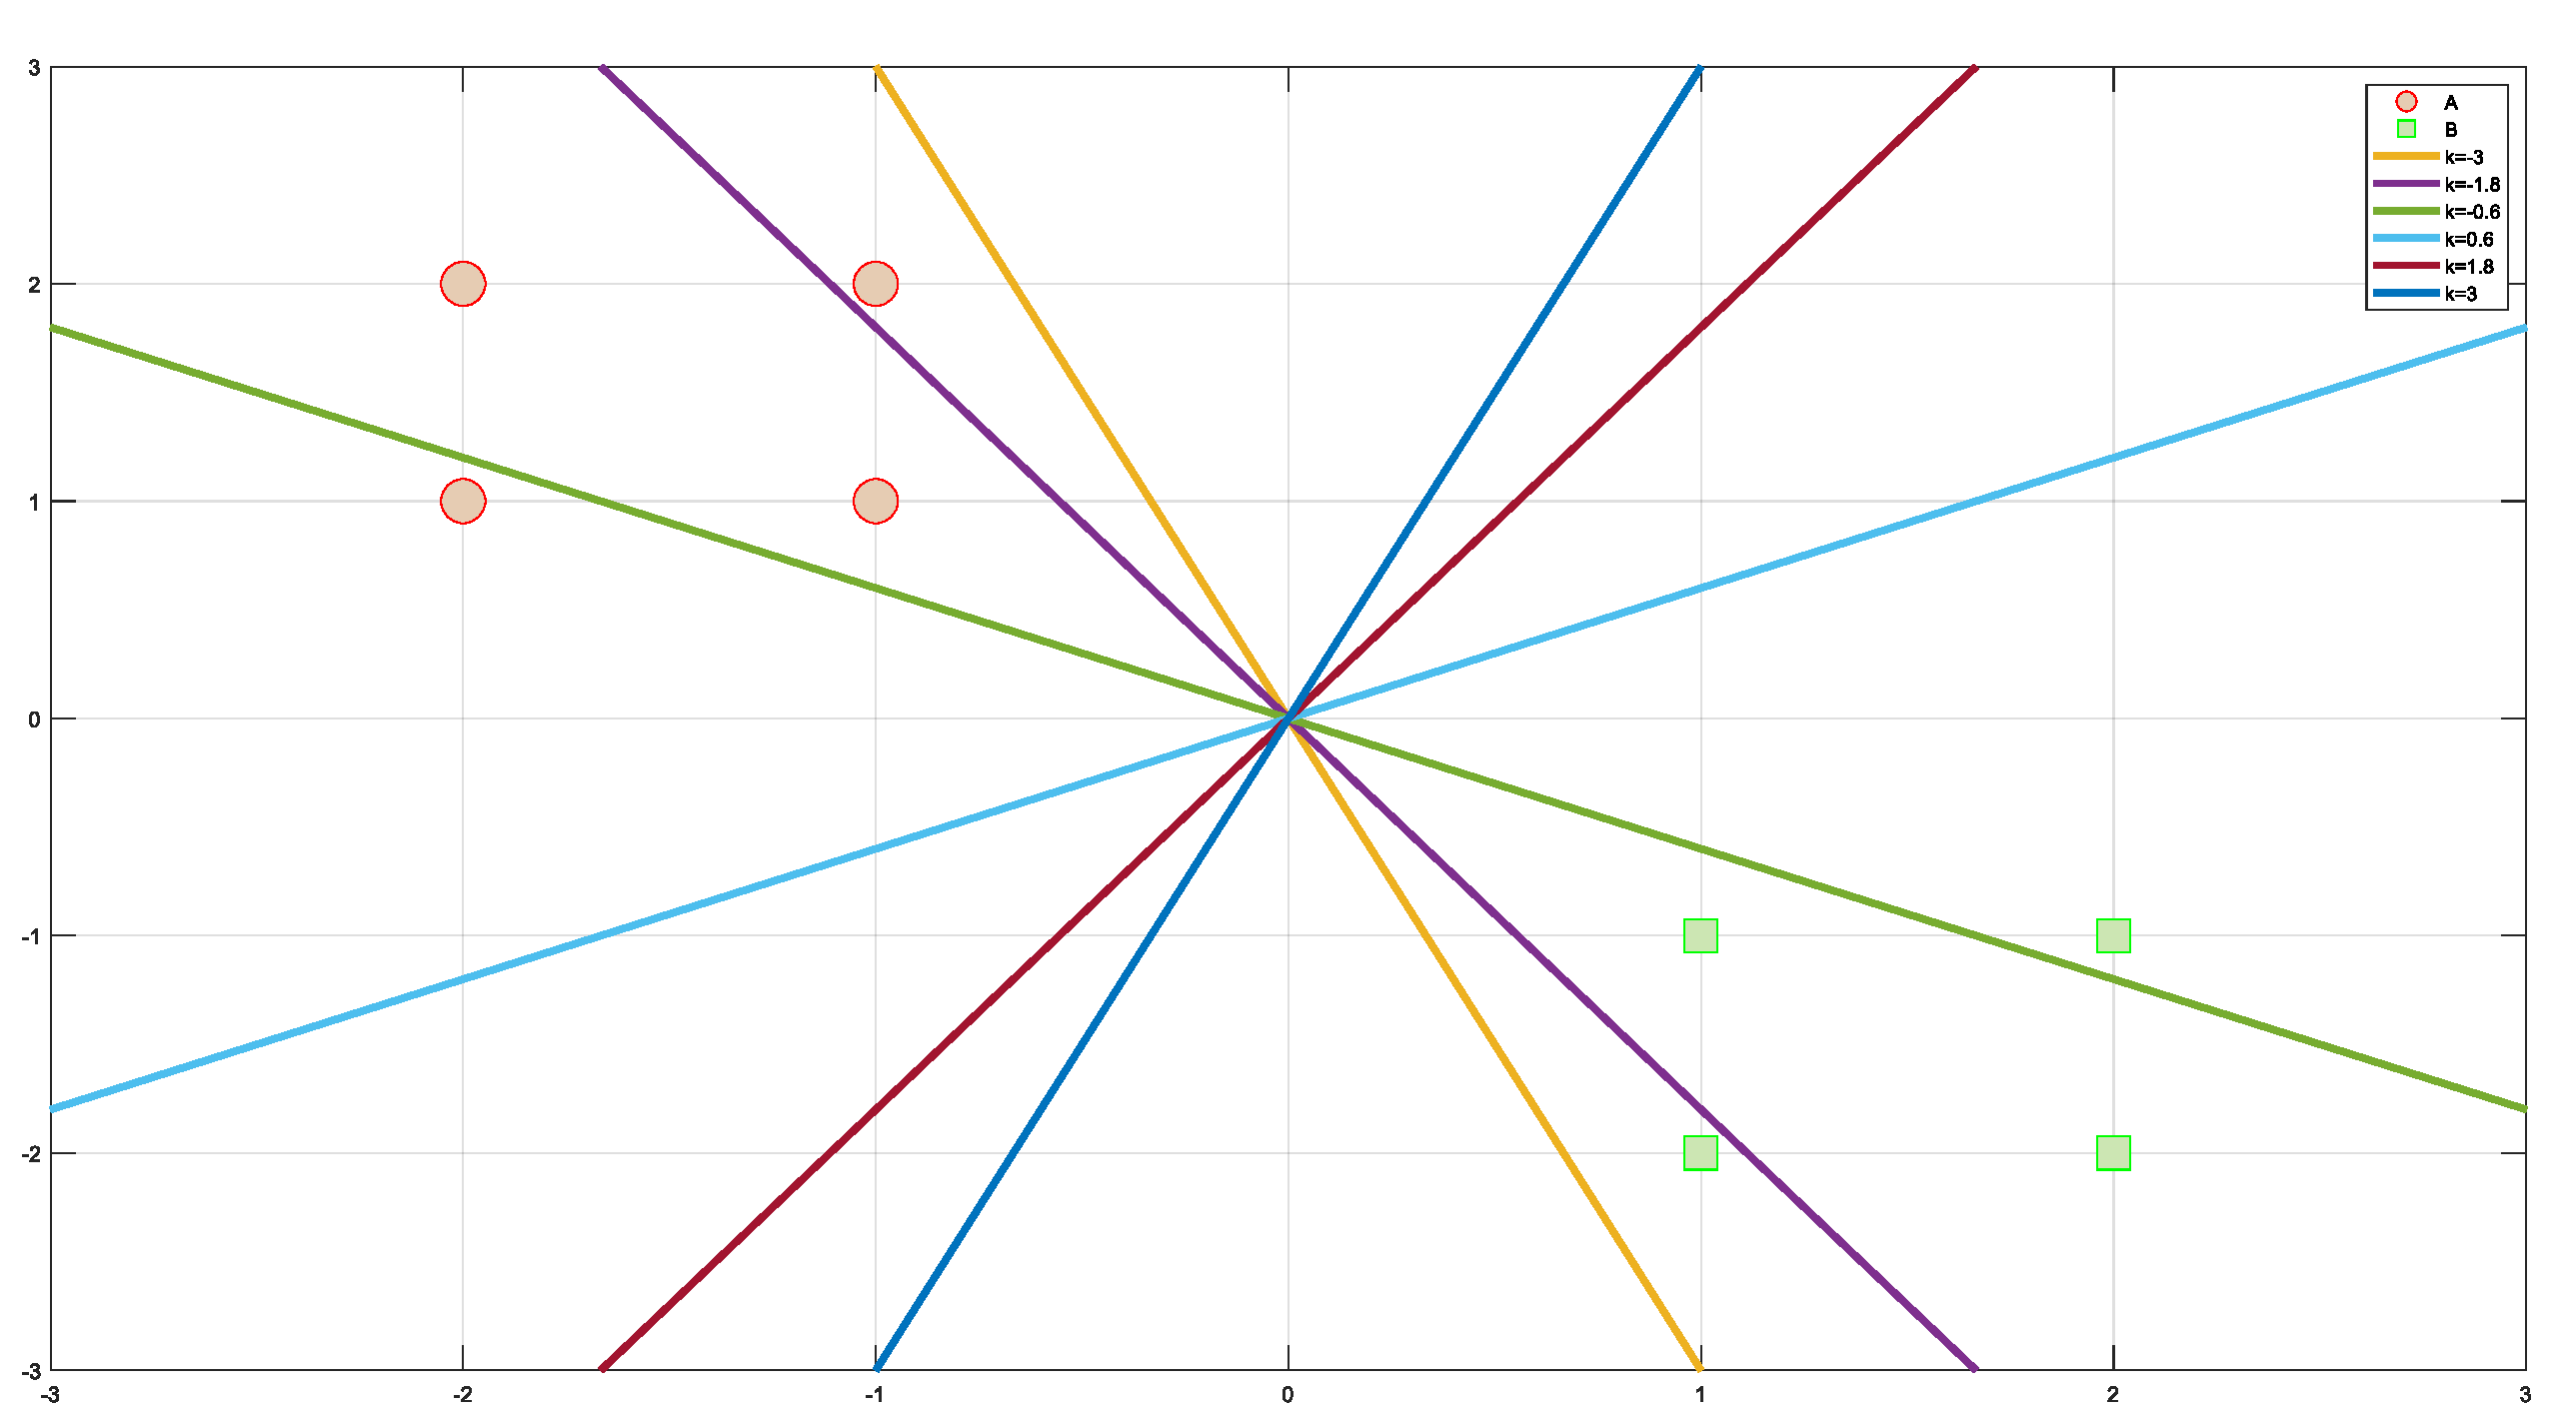
\includegraphics[scale=0.2]{pic/act1.pdf}
        \caption{调整动作(这里是斜率$k$)来使得直线将A和B分为两个类别.}
    \end{figure}
\end{frame}


\begin{frame}{移步到BNNs中}
    \footnotesize
    在BNNs中, 由于二值参数的非连续性. 将其看做是动作的更新而不是通过梯度来更新是很自然的. 当然与图\ref{fig:maze}的问题比起来我们的模型将更加复杂. 因为在迷宫问题中, 机器人只有一个动作需要更新: 即上下左右中的一个. 而对于一个参数矩阵来说, 所有的矩阵元素都将可能是我们需要更新的动作. 我们可以看做是向前或向后或原地不动. 就如同人类的婴儿学习走路一样, 我们应该如何让自身的关节相互协调, 以达到平稳行走的目的.
    \par 假设$\mathcal{D} =\left\{ \mathrm{X},\boldsymbol{y} \right\} $是包含了输入和输出的数据集. 一个BNNs模型被定义如下:
    \begin{equation}
        \mathcal{F} =\mathcal{F} \left( \mathrm{X};\left[ \mathrm{W}_{b}^{1},\mathrm{W}_{b}^{2},\mathrm{W}_{b}^{3} \right] \right),
    \end{equation}
    \begin{equation}
        \mathcal{L} =\mathcal{L} \left( \mathcal{F} \left( \mathrm{X} \right) ,\boldsymbol{y} \right).
    \end{equation}
\end{frame}


\begin{frame}{移步到BNNs中}
    \footnotesize
    为了方便, 我们定义二值矩阵为$2\times 2$的矩阵. 那么可能让BNN学会平稳\textcolor{red}{行走}的策略可以由下图表示:
    \begin{figure}
        \centering
        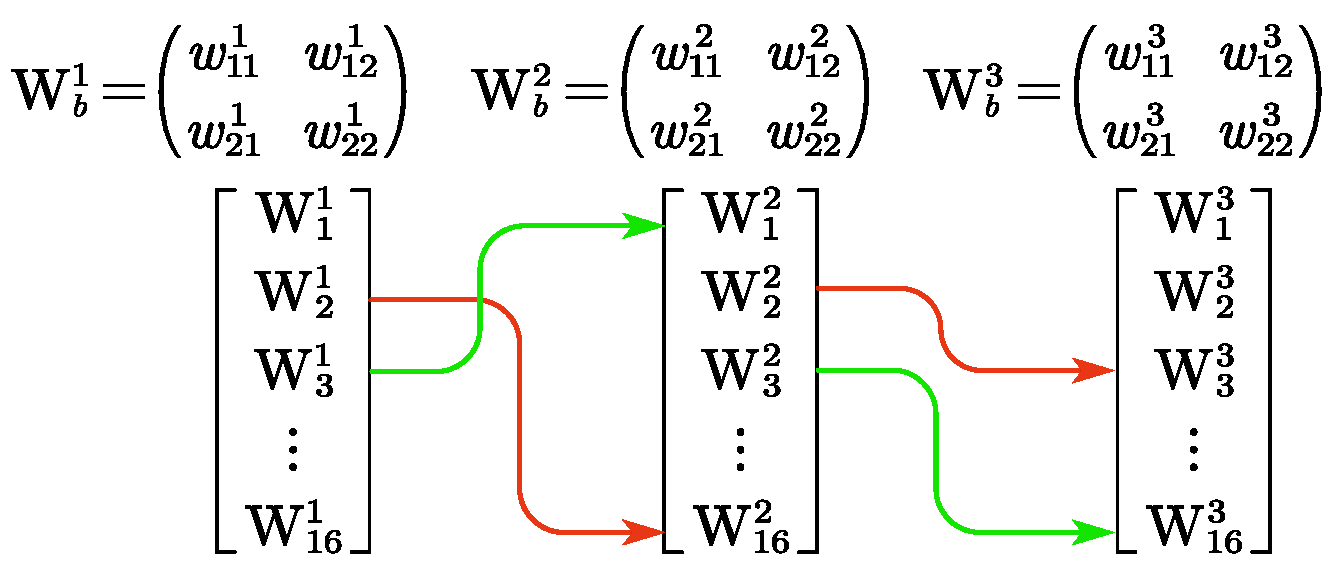
\includegraphics[scale=0.4]{pic/w3.pdf}
        \caption{不同颜色的线条表示我们的不同策略}
    \end{figure}
\end{frame}

\begin{frame}{可行性分析}
    \footnotesize
    \begin{textbox}{理论的支撑}
        据文献\cite{1998Reinforcement}记载, 早在$1954$年 Minsky \footnotemark 首次提出\textcolor{red}{强化}一次的概念. 并且确立了\textcolor{red}{试错}是强化学习的核心机制. 早期的强化学习是为了求解最优控制问题, 并开发了\textcolor{red}{动态规划}和\textcolor{red}{马尔科夫决策过程}的策略迭代方法. $1988$年 Minh 提出时序差分算法\cite{mnih2015human}, 并且于$1989$年, Watking提出了Q-Learning\cite{watkins1992q}算法, 并给出了算法的收敛性证明, 强化学习理论开始逐渐开始完备.
    \end{textbox}
    \begin{textbox}{实践的探索}
        目前, 已有不少研究使用强化学习的方式自动生成ANN的结构(\cite{jaques2017tuning, baker2016designing, zoph2016neural}等). Aenugu 提出了一种使用强化学习训练脉冲神经网络的方法\cite{aenugu2020training}. James 等人提出了一种使用学习自动机\cite{lindsay2020novel}来训练ANN的方法, 而不需要误差的反向传播. Lazarus\cite{lazarus2022deep}使用BNNs替换DQN中的ANN, 提出了一种BQN-L算法, 但是该算法仍然没有放弃用全精度计算梯度的思想. Sourabh 等人提出了一种使用策略梯度(PG)训练神经网络的方案\cite{2017Training}. 该方法重心在对神经元激活值(\textcolor{red}{而不是直接对权重})的建模, 通过另一个ANN的学习来导出梯度. 
    \end{textbox}
    \footnotetext{\tiny{Minsky是人工智能之父, 并获得1969年图灵奖}}
\end{frame}


\begin{frame}{强化学习算法}
    \footnotesize
    强化学习大约可以分为有模型和无模型的强化学习算法:
    \begin{figure}
        \centering
        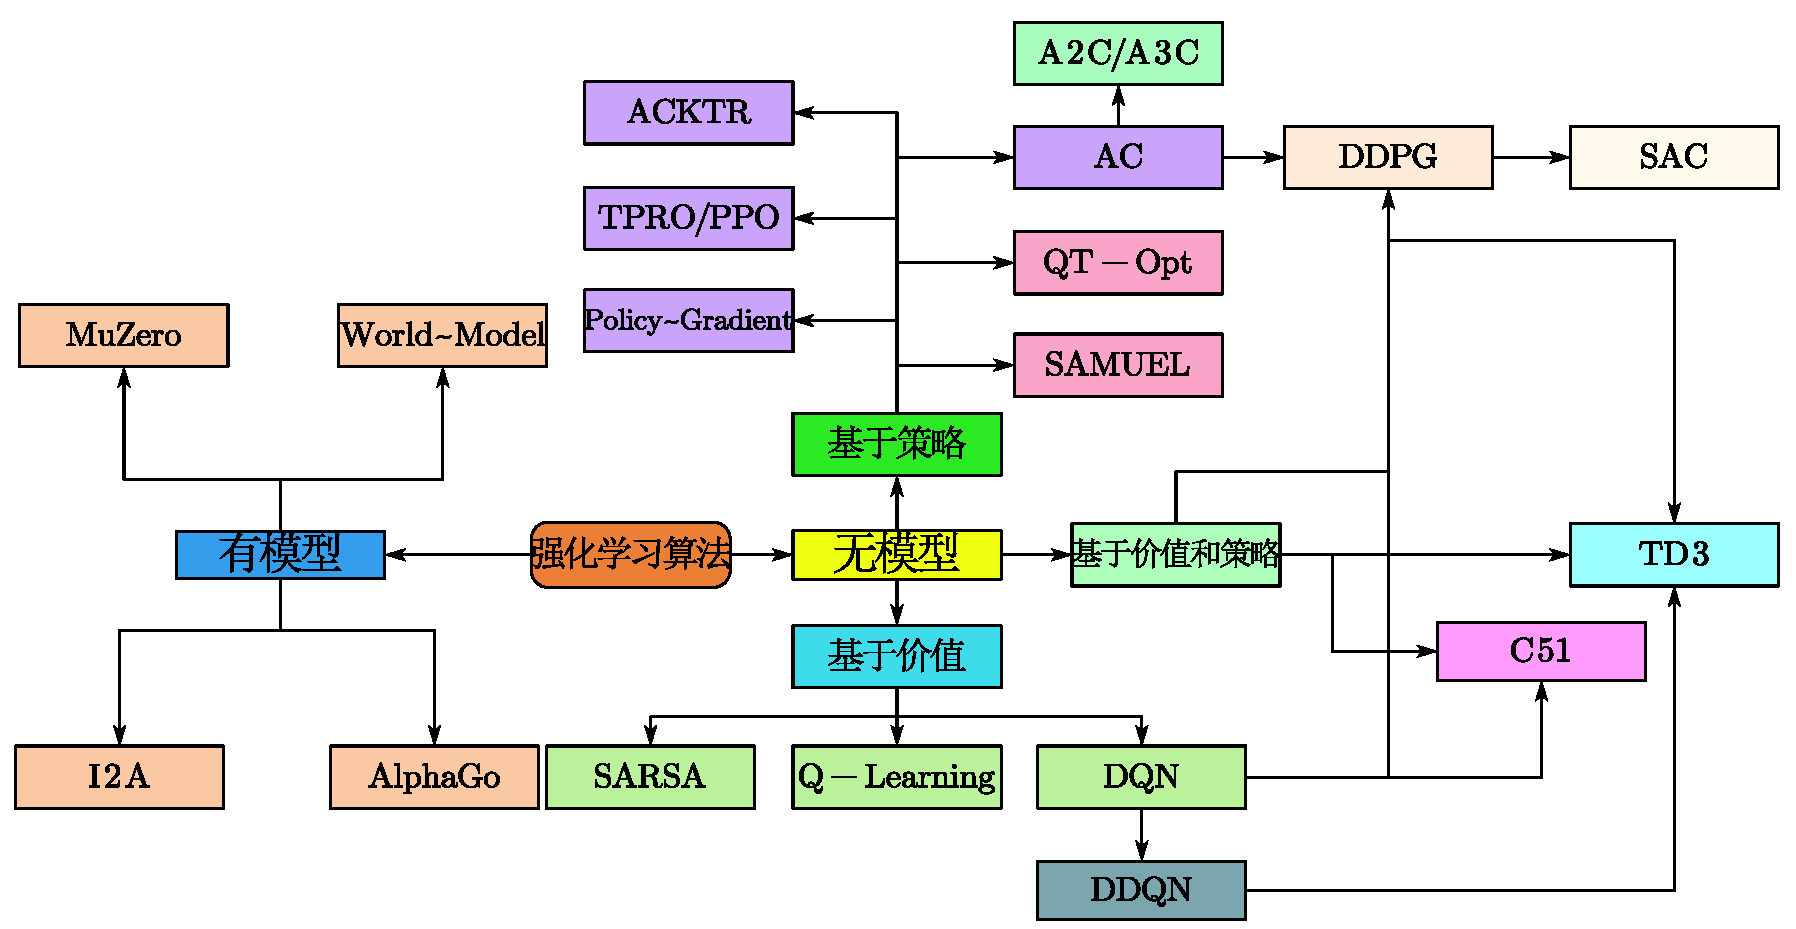
\includegraphics[scale=0.3]{pic/ags.pdf}
        \caption{常见强化学习算法分类}
    \end{figure}

\end{frame}



\begin{frame}{有模型和无模型的区别}
    \footnotesize
    下图展示了有模型和无模型的区别:
    \begin{figure}
        \centering
        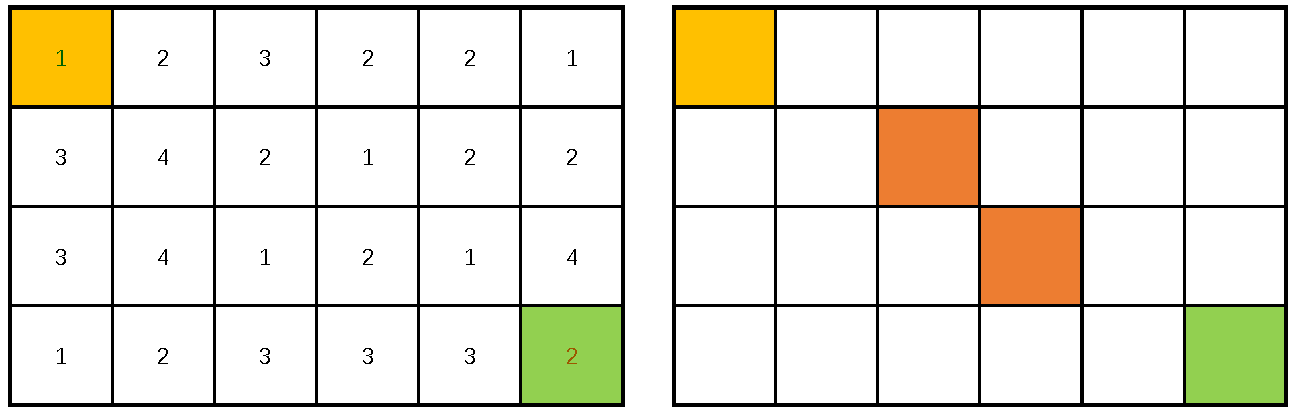
\includegraphics[scale=0.35]{pic/dprl.pdf}
        \caption{有模型 \& 无模型}
    \end{figure}
    假设网格的值用$\mathrm{M}$表示, $\mathrm{D}_{ij}$表示到达$i$行$j$列时的最大奖励. 那么状态转移方程可以表示如下:
    \begin{block}{状态转移方程}
        \begin{equation}
            \mathrm{D}_{ij}=\max \left( \mathrm{D}_{i-1,j}, \mathrm{D}_{i,j-1}+\mathrm{M}_{ij} \right) 
        \end{equation}
    \end{block}
\end{frame}

\begin{frame}{策略梯度定理}
    \footnotesize
    % \kaishu
    \begin{define}[{策略与奖励}]
        我们定义在状态$s$下动作执行$a$的概率为$\pi_\theta(a|s)$. 这种策略称为随机策略. 我们用$r_t$表示在$t$时刻的奖励, $R_t$表示从$0$时刻到$t$时刻的总奖励和. 并用$\gamma$表示折扣因子, 这是一个超参数, 是我们对未来的获得奖励的衰减值系数.
    \end{define}
    
    \begin{define}[{价值函数}]
        \begin{textbox}{{\footnotesize\textcolor{red}{状态}价值函数}}
            \begin{equation}
                V_{\pi}(s) \doteq \mathbb{E}_{\pi}\left[R_{t} \mid s_{t}=s\right]=\mathbb{E}_{\pi}\left[\sum_{k=0}^{\infty} \gamma^{k} r_{t+k+1} \mid s_{t}=s\right]
            \end{equation}
        \end{textbox}
        \begin{textbox}{\footnotesize\textcolor{red}{状态-动作}价值函数}
            \begin{equation}
                Q_{\pi}(s, a) \doteq \mathbb{E}_{\pi}\left[R_{t} \mid s_{t}=s, a_{t}=a\right]=\mathbb{E}_{\pi}\left[\sum_{k=0}^{\infty} \gamma^{k} r_{t+k+1} \mid s_{t}=s, a_{t}=a\right]
            \end{equation}
        \end{textbox}
    \end{define}
    
\end{frame}

\begin{frame}{策略梯度定理}
    \footnotesize
    \begin{thm}[策略梯度定理\cite{1998Reinforcement}]
        强化学习的学习目标是最大化奖励:
        \begin{equation}
            J\left(\pi_{\theta}\right)=\mathbb{E}_{\tau \sim \pi_{\theta}}[R(\tau)]=\mathbb{E}_{\tau \sim \pi_{\theta}}\left[\sum_{t=0}^{\mathrm{T}} R_{t}\right]=\sum_{t=0}^{\mathrm{T}} \mathbb{E}_{\tau \sim \pi_{\theta}}\left[R_{t}\right]
        \end{equation}
        那么我们有:
        \begin{equation}
            \nabla J(\theta)=\mathbb{E}_{\tau \sim \pi_{\theta}}\left[\sum_{t^{\prime}=0}^{T} \nabla_{\theta} \log \pi_{\theta}\left(a_{t^{\prime}} \mid s_{t^{\prime}}\right) \gamma^{t^{\prime}} \sum_{t=t^{\prime}}^{T} \gamma^{t-t^{\prime}} R_{t}\right]
        \end{equation}
        这是策略梯度的基本形式.
    \end{thm}
    
\end{frame}

\begin{frame}{需要克服的问题}
    \footnotesize
    \begin{enumerate}
        \item 与一般的强化学习模型不同, 训练BNNs的过程更像是多智能体学习, 而不是简单的只有一个机器人走迷宫问题. 然而关于多智能体学习的研究还相对较少.
        \item 没有一套合适的二值计算工具, 能让计算过程全部以逻辑值($0\&1$)进行. 而(如MATLAB等)直接将矩阵元素看做是$0\&1$时, 它的数据类型仍然是一个浮点型或者整型.
        \item BNNs不是一种ANN模型, 而是一类ANN模型. 新的训练方法需要尽可能多的能够迁移到其它ANN框架.
    \end{enumerate}
\end{frame}

\section{计划进度}

\begin{frame}{时间表}
    \begin{figure}
        \centering
        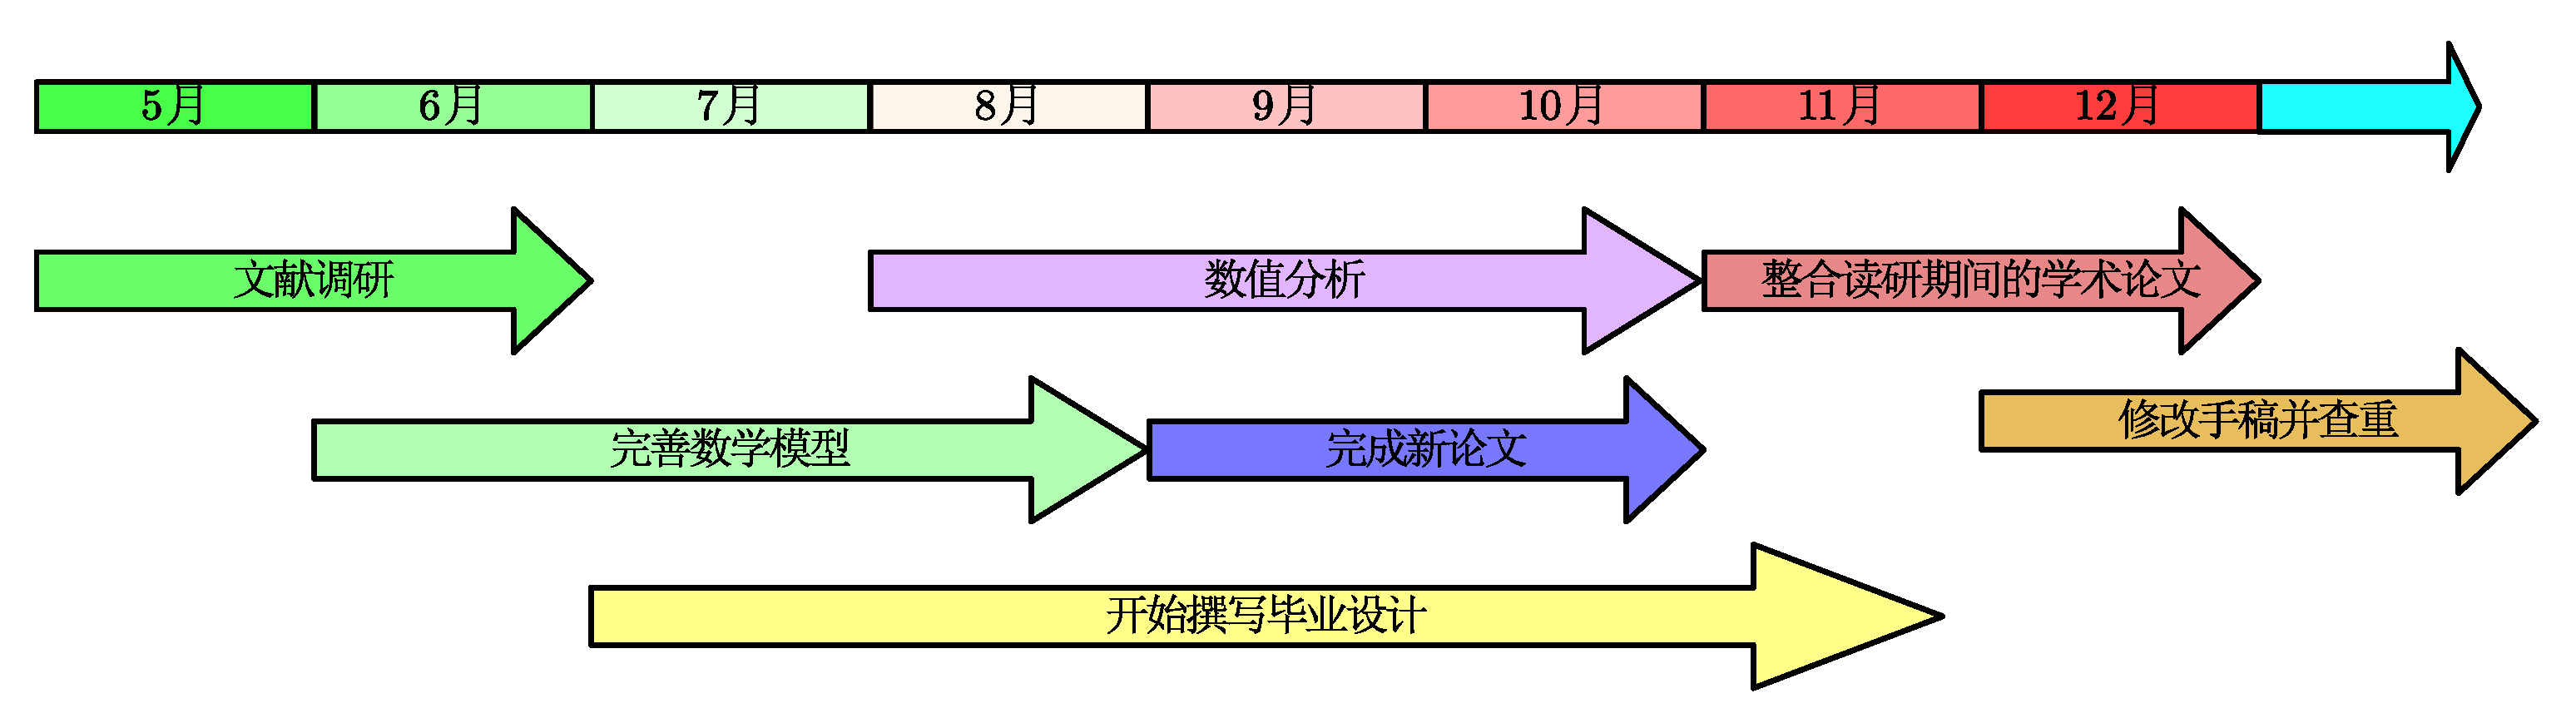
\includegraphics[scale=0.2]{pic/mytime.pdf}
    \end{figure}
\end{frame}


\section{参考文献}

\begin{frame}[allowframebreaks]
    \tiny
    \bibliography{ref}
    \bibliographystyle{unsrt}
\end{frame}

\begin{frame}
    \begin{center}
        {\Huge\calligra Thanks!}
    \end{center}
\end{frame}

\end{document}